\chapter{Performance Evaluation} \label{chp_perf_eval}
\section{Maximum System Efficiency and Minimum Access Delay} 	\label{sec_max_min}
With the system efficiency given in equation \ref{eff_def}, we take the derivative with respect to $\tau$, and find the extreme point, $\tau^\star = M/n$. Since $\tau\in [0,1]$, $\tau^\star = min\lbrace 1,M/n\rbrace$. 
What we care is when $n$, the number of contending stations, is large, i.e., $\tau^\star = M/n$. 
Then the system efficiency is
\begin{align}
\textit{eff}\ (\tau^\star) = (1-\frac{1}{n})^{n-1} 
\label{equ_max_eff}
\end{align}
Then the maximum $n_s$ is easy to generate.
\begin{align}
\label{equ_max_ns}
E[n_s]^\star = M \cdot \textit{eff}\ (\tau^\star) = M(1-\frac{1}{n})^{n-1} 
\end{align}
Thus the limit of system efficiency, based on infinite $n$, is
\begin{align}
\label{eff_limit}
\lim_{n\rightarrow \infty}\textit{eff}\ (\tau^\star) = \lim_{n\rightarrow \infty}(1-\frac{1}{n})^{n-1} =\frac{1}{e} 
\end{align}

\begin{figure}[!ht]
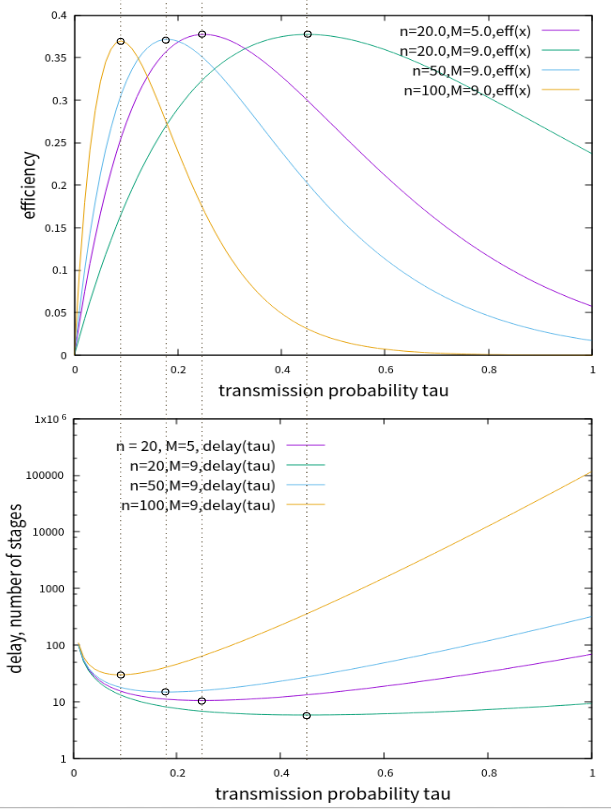
\includegraphics[scale=0.64]{./figure/chp4/max_min.png}
\caption{Efficiency and access delay versus transmission probability $\tau$}
\label{fig_eff_def}
\end{figure}


With the delay analysis given in \ref{equ_delay}, we also take the derivative with respect to $\tau$, and find the extreme point, $\tau^\star = M/n$. Again, $\tau^\star = min\lbrace 1, M/n\rbrace$. 
When $n\geq M$, the minimum access delay is 
\begin{align}
\label{equ_min_delay}
D(\tau^\star) = \frac{n}{M(1-\frac{1}{n})^{n-1}}.
\end{align}

From above analysis, we find that the maximum system efficiency and minimum access delay are both obtained by the same transmission probability $\tau^\star = min\lbrace 1, M/n\rbrace$.
What's more, system efficiency is independent with $M$, number of RUs for random access in a stage, while $M$ affects access delay. 
The larger $M$ is, the shorter the access delay will be. 
It indicates that when AP allocates RUs for random access, the AP could allocates as many as possible, only if the channel of the RU is sensed idle. 
This rule will be more explained in next section.

Figure \ref{fig_eff_def} is plotted corresponding to equation \ref{eff_def} and \ref{equ_delay}.
Consistent to the analysis above, the figure shows that the maximum system efficiency is independent of number of RUs for random access when $n\geq M$, and approaching to $1/e$ with $n$ increasing. 
What's more, the optimal transmission probability $\tau$ of system efficiency and access delay is consistent with each other, which also validates the analysis. 

According to equation \ref{tau_general} and \ref{p_ax}, transmission probability $\tau$ is dependent on system parameters, $M$ (RUs for random access in a stage), $W_0$ (initial contention window) $m$ (backoff levels) or $W_m$ (the maximum contention window) and $n$ (number of stations in the network).
The only way to approach optimal performance is to employ adaptive techniques to tune the system parameter set $\lbrace M, W_0, W_m \rbrace$ on the basis of the estimated value of $n$.
In the following section, we will evaluate the performance corresponding to different system parameters sets and propose the rules to tune the system parameter sets so that the transmission probability $\tau$ approach the optimal transmission probability, $\tau^\star$, which means both system efficiency and delay approach the optimal. 

\section{Rules of Parameter Configuration} 	\label{sec_perf_eval}
We have estimated the maximum system efficiency and minimum access delay in the previous section. Then we evaluate the metrics, $n_s$ (number of stations who succeed in contending in a stage), system efficiency and $D$ (access delay), under various parameter sets. 
With above analysis, we could evaluates transmission probability under various parameter sets, since the optimal transmission probability $\tau^\star$ means both maximum system efficiency and minimal access delay.

At last, we propose rules for configuring the parameter set $\lbrace M, OCW_{min}, OCW_{max}\rbrace$.

\subsection{RUs for Random Access $M$}
\label{M}
Equation \ref{equ_max_eff} indicates that $M$, the number of RUs for random access, has nothing to do with maximum system efficiency. 
However, larger $M$ is better for $n_s$ and $D$ according to equation \ref{equ_max_ns} and \ref{equ_min_delay}. More explaination are given later to validate the statement. 

In figure \ref{fig_n_M_eff}, the maximum system efficiency is the same. 
The difference is "when" the optimal point will be. 
For larger $M$, the optimal number of stations is larger, given by $M/n$. It is also intuitive.

\begin{figure}[!h]
\centering
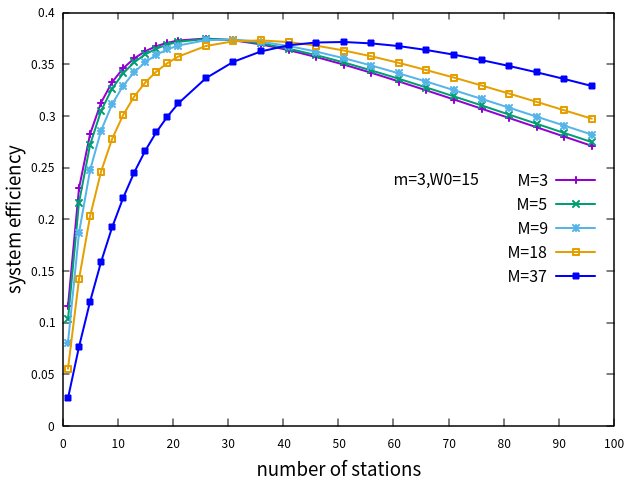
\includegraphics[scale=.85]{./figure/n_M_eff_perf.png}
\caption{System efficiency versus number of stations}
\label{fig_n_M_eff}
\end{figure}

\begin{figure}[!h]
\begin{subfigure}{\textwidth}  
\centering
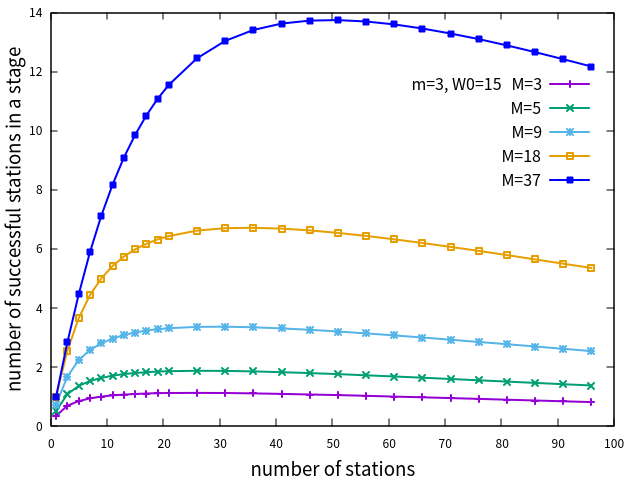
\includegraphics[scale=.85]{./figure/n_M_ns_perf.png}
\caption{Number of successful stations in a single stage versus number of stations}
\label{fig_n_M_ns}
\end{subfigure}

\begin{subfigure}{\textwidth}  
\centering
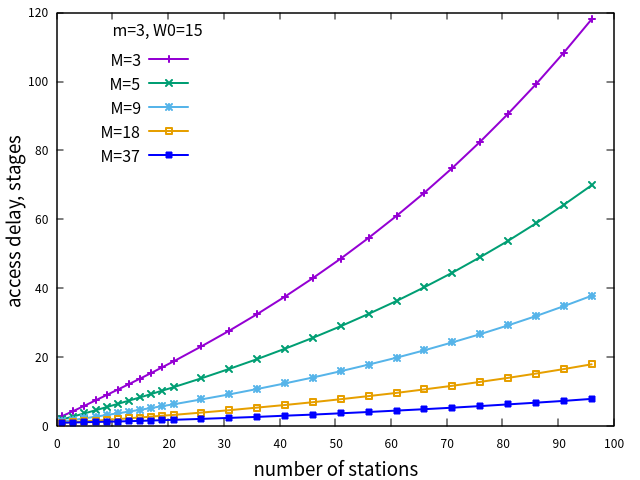
\includegraphics[scale=.85]{./figure/n_M_delay_perf.png}
\caption{Access delay versus number of stations}
\label{fig_n_M_delay}
\end{subfigure}
\caption{Configure $M$}
\end{figure}

In figure \ref{fig_n_M_delay}, the larger $M$ will linearly decrease the access delay of station. The figure is consistent with the equation \ref{equ_min_delay}. 

More practically, we present the number of successful stations in a single stage versus number of stations in figure \ref{fig_n_M_ns}.
While the maximum system efficiency is the same with different $M$, the actually number of stations who succeed contending in a single stage is much different, which corresponds to equation \ref{equ_max_ns}. 
The optimal value of number of successful stations in a single stage is proportional to $M$. 
Above all, when AP allocates RUs for random access, the AP will sense channels first then allocates as many RUs, which are sensed idle, for random access as possible.



\subsection{Initial and max Contention Window $(OCW_{min}, OCW_{max})$}
\label{contend_window}
Different from legacy 802.11 where backoff mechanism is pre-set in hardware of stations, the initial and maximum contention window $(OCW_{min}, OCW_{max})$ are allocated in beacon frame sent by AP. 
Thus, the configuration of backoff mechanism becomes dynamic, which means that it could be configured according to the scenario, especially the number of stations.
With the $M$ being determined as large as possible, it is more complicated algorithm to adaptive tune $OCW_{min}, OCW_{max}$ so that transmission probability approaches optimal value.
Since $\tau$ is determined by solving equations \ref{tau_general} and \ref{p_ax}, it is hard to give a expression of $\tau$ determined by system parameters $W_0$ and $W_m$.
However, we could find the rules by checking a variety of parameter sets.

% figures
\begin{figure}[!t]
\centering
%subfigure
\begin{subfigure}{\textwidth}
\centering
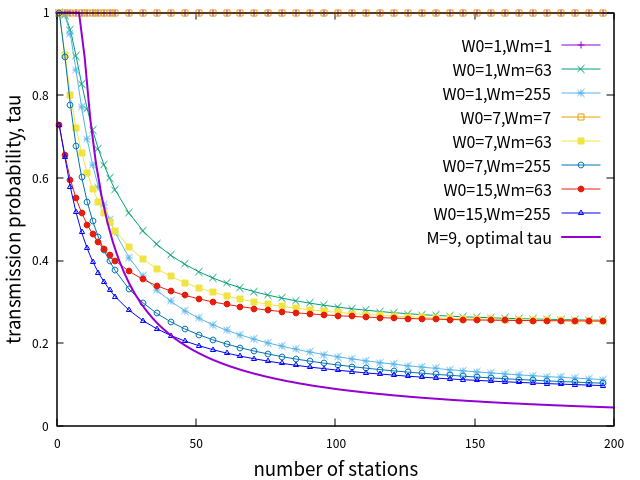
\includegraphics[scale=.85]{./figure/chp4/M9/n_tau_perf_M9_x200.png}
\caption{Case 1, given $M=9$}
\label{fig_tau_n_M9}
\end{subfigure}
%subfigure
\begin{subfigure}{\textwidth}
\centering
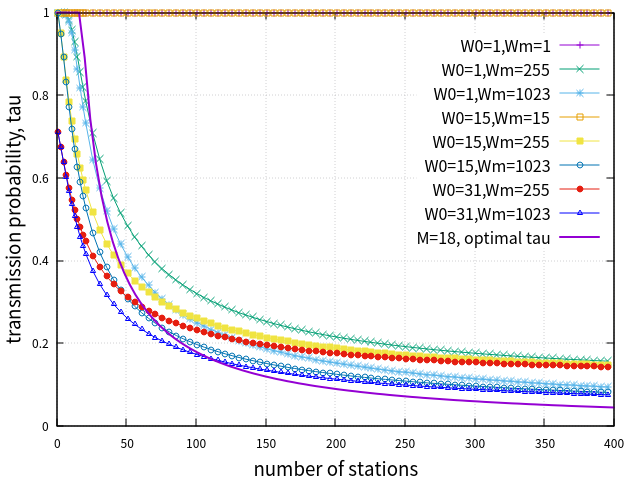
\includegraphics[scale=.85]{./figure/chp4/M18/n_tau_perf_M18_x400.png}
\caption{Case 1, given $M=18$}
\label{fig_tau_n_M18}
\end{subfigure}
%caption
\caption{Transmission probability versus number of stations}
\label{fig_tau_n}
\end{figure}

Figure \ref{fig_tau_n} shows case 1 ($M=9$) and case 2 ($M=18$), from both of which we could generalize some rules between $\tau$ and parameters $OCW_{min}, OCW_{max}$.
In the figure, the purple line without point is the optimal $\tau$, which is given according to $\tau^\star = min\lbrace 1, M/n \rbrace$.
As stated above, we need to find a tuning of $OCW_{min}, OCW_{max}$ so that $\tau$ approaches the optimal line. The rules are listed following.

Firstly, the $OCW_{min}$, namely $W_0$, determines the start of the line of $\tau$. The larger $W_0$ is, the lower transmission probability will start at $n=1$.
A special situation is when $W_0<M$, $\tau=1$ at $n=1$. 
That's why cases in figure \ref{fig_tau_n} have two different start points.
For optimal transmission probability $\tau^\star$, when $n \leq M$, $\tau^\star = 1$. 
A special case of $m=0$, which means $W_m=W_0$, results in constant transmission probability equal to 1, which is perfect match with $\tau^\star$ at $n\leq M$.
Thus, if given $n\leq M$, the optimal configuration will be $OCW_{max}= OCW_{min} < M$. 


Secondly, $W_m$ determines limit of the $\tau$, i.e., where the line will converge. 
Lines with the same $W_m$ will converge to a same value. 
To see the tendency of lines, I draw the two figures \ref{fig_tau_n_M9} and \ref{fig_tau_n_M18} with $n$ in range $[0,200]$ and $[0,400]$ respectively. 
And both the two figures validate the above statement.
And larger $W_m$ is closer to optimal transmission probability when $n$ is large. 
When $m=0$, $\tau$ will not change with $n$, which is consistent with equation \ref{tau_W0}.
For those $m>0$, the curve will be convex. It is intuitive that with the number of stations increasing, the collision probability will increase, thus contention window increase. 


% figures
\begin{figure}[!t]
\centering
\begin{subfigure}{\textwidth}
\centering
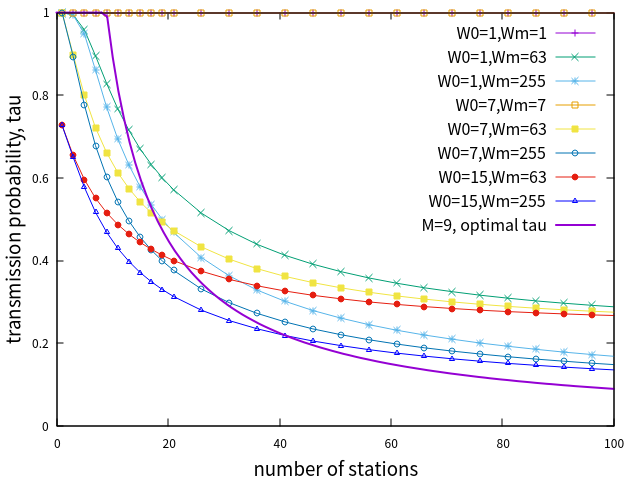
\includegraphics[scale=.85]{./figure/chp4/M9/n_tau_perf_M9_x100.png}
\caption{Case 1, given $M=9$}
\label{fig_tau_n_M9_detail}
\end{subfigure}

\begin{subfigure}{\textwidth}
\centering
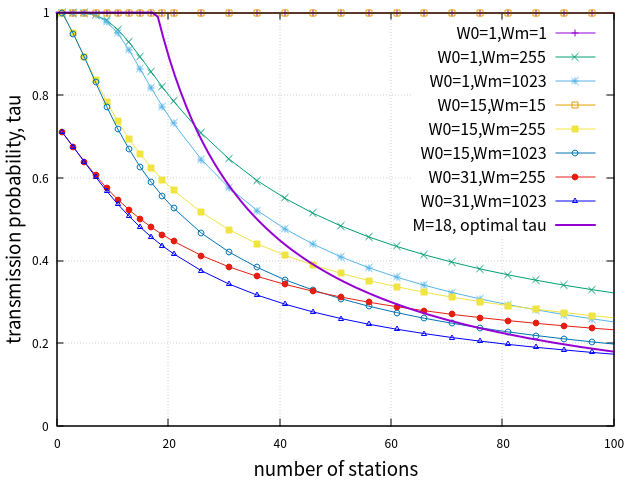
\includegraphics[scale=.85]{./figure/chp4/M18/n_tau_perf_M18_x100.png}
\caption{Case 1, given $M=18$}
\label{fig_tau_n_M18_detail}
\end{subfigure}

\caption{Details of transmission probability versus number of stations when $n\leq 100$}
\label{fig_tau_n_detail}
\end{figure}

Then, we draw two figures with x axis range $[0,100]$ to find more rules as in figure \ref{fig_tau_n_detail}. 
From the two figures \ref{fig_tau_n_M9_detail} and \ref{fig_tau_n_M18_detail} we find another rule that if $W_0=1$ which is the minimum value, there will be a flat start of $\tau$.
What's good is that the flat start is closer to $\tau^\star$ when $n\leq M$.

Based on above observation, we find conclude that $W_0$ has significant influence on small $n\leq M$, while $W_m$ affects $n$ is large or $n>M$. 
Afterwards, in the next two subsections, we check the system efficiency and access delay under different parameter sets of $\lbrace W_0, W_m \rbrace$, with which we could find explicit relationship between the parameter and performance.




\subsubsection{Configure $OCW_{max}$}

\begin{figure}[!t]
\centering
\begin{subfigure}{\textwidth}  
  \centering  
  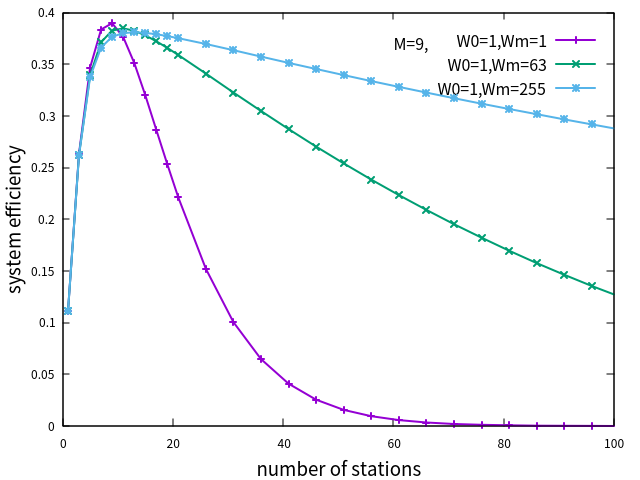
\includegraphics[scale=0.85]{./figure/chp4/M9/n_eff_perf_W01.png}  
    \caption{System efficiency versus number of stations}   
    \label{fig_n_eff_Wm}
\end{subfigure}   

\begin{subfigure}{\textwidth}
	\centering
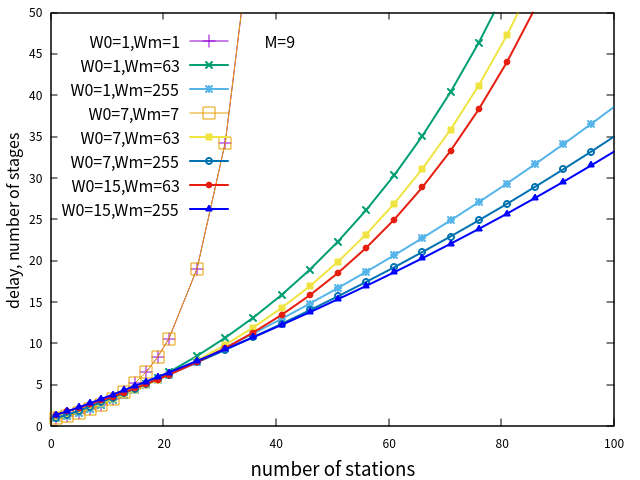
\includegraphics[scale=.85]{./figure/chp4/M9/n_delay_perf.png}
\caption{Access delay versus number of stations}
\label{fig_n_delay_Wm}
\end{subfigure}
\caption{Example of Configuring $OCW_{max}$, given $M=9$}
\end{figure}

With above rough rules, we estimate the effects of $OCW_{max}$ first by setting different $OCW_{max}$ while given $OCW_{min}=1$ and $M=9$.
It is because small $OCW_{min}$ is good for situation of small $n$.
Actually the data we use to generate the figures are the same as that for figure \ref{fig_tau_n_M9}. For figure \ref{fig_n_eff_Wm}, we display three of them to clearly show relationship between system efficiency and $OCW_{max}$.
And from the figure, it is apparent that larger $OCW_{max}$ is better for system efficiency. 
The result corresponds to the second rule we obtain when estimating the transmission probability $\tau$.
What's more, the access delay also validates the same result. And since we use the same data with that in figure \ref{fig_tau_n_M9}, we find that the lines which converge in figure \ref{fig_tau_n_M9} also have the same tendency in figure \ref{fig_n_delay_Wm}. 

As stated in last section that $OCW_{max}$ has significant influence on situation of large $n$, $n$ is number of contending stations. With increasing $n$, larger $OCW_{max}$ will obtain larger gain. 
Therefore, we have a rule that the larger $OCW_{max}$, the better.



\subsubsection{Configure $OCW_{min}$}

\begin{figure}[!t]
\centering
\begin{subfigure}{\textwidth}  
  \centering  
  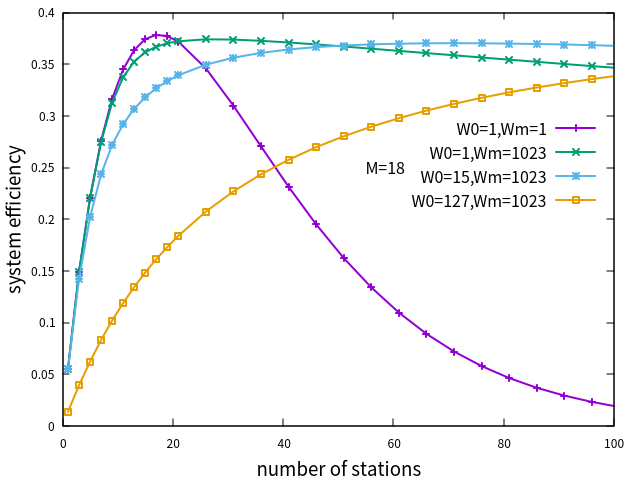
\includegraphics[scale=0.85]{./figure/chp4/M18/n_eff_perf_Wm1023.png}  
    \caption{System efficiency versus number of stations}   
    \label{fig_n_eff_W0}
\end{subfigure}   

\begin{subfigure}{\textwidth}
	\centering
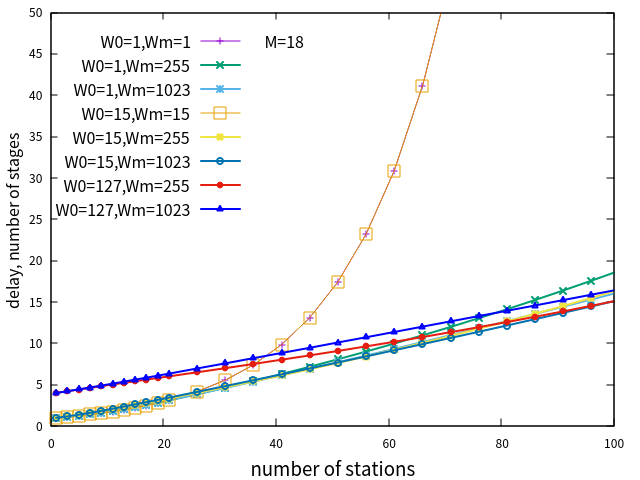
\includegraphics[scale=.85]{./figure/chp4/M18/n_delay_perf.png}
\caption{Access delay versus number of stations}
\label{fig_n_delay_W0}
\end{subfigure}
\caption{Example of Configuring $OCW_{min}$, given $M=18$}
\end{figure}

Similarly, to estimate the relationship between performance and $OCW_{min}$, we compare the performance between different $OCW_{min}$ while given fixed $OCW_{max}=1023$, which has been validated that large $OCW_{max}$ is better, and $M=18$. 
Firstly, we claimed in section \ref{contend_window} that $W_0=W_m\leq M$ is the perfect configuration in situation of $n\leq M$. It is again validated here that it has the maximum system efficiency and minimum access delay in situation of $n\leq M$. 
Secondly, since $OCW_{min}$ determines the start of line, i.e., $n=1$, it has significant influence on small $n$.
From figure \ref{fig_n_eff_W0} and \ref{fig_n_delay_W0}, we find larger $OCW_{min}=127$ has lower system efficiency and longer access delay. And as stated before, $W_0=15$ has close performance with $W_0=1$ since $W_0<M$ will be similar for situation of small $n$.

Therefore, we generate a rule that the smaller $OCW_{min}$, the better.
For a special situation that $n\leq M$, we could configure $OCW_{min}=OCW_{max}<M$, which will result in perfect performance. 
However, larger $OCW_{max}$ smaller $OCW_{min}$ is closely approach to optimal performance.

\subsection{Rules for configuring $\lbrace M, OCW_{min}, OCW_{max} \rbrace$}
Above two previous subsections, we could conclude rules of configuring the parameter set $\lbrace M, OCW_{min}, OCW_{max} \rbrace$ for obtaining best performance for all $n$. 
\begin{itemize}
\item[Rule 1] Large $M$
\item[Rule 2] $OCW_{min}, OCW_{max}$
	\begin{itemize}
	\item small $OCW_{min}$ and large $OCW_{max}$
	\item If given $n\leq M$
	\begin{itemize}
		\item $OCW_{max}=OCW_{min}<M$
	\end{itemize}
	\end{itemize}
\end{itemize}

%After we propose the rules of configuring the parameter set $\lbrace M, OCW_{min}, OCW_{max} \rbrace$, we run another analysis with typical group parameter sets which validate our rules.

%From figure \ref{fig_n_ns_val}, larger $M = 18$  results in larger $n_s$, number of successful stations in a single stage, than $M=9$. Thus, $M$ is as large as possible.
%Then given a $M=18$ as an example, smaller $W_0 = 7$ and larger $m = 7$ have better performance than other parameter sets when $n>M$.
%
%For the system state that $n\leq M$, $n_s$ and access delay of $m=0,W_0 = 7$ is the best case among all the parameter sets. It is because the transmission probability under such condition reaches the optimal value as in figure \ref{fig_n_tau}.  

%\begin{figure}[!ht]
%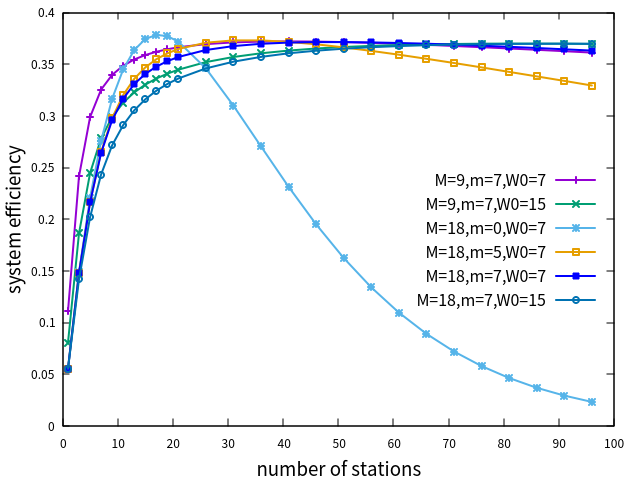
\includegraphics[scale=.54]{./figure/n_rule_eff_perf.png}
%\caption{System efficiency versus number of stations}
%\label{fig_n_eff_val}
%\end{figure}
%
%\begin{figure}[!ht]
%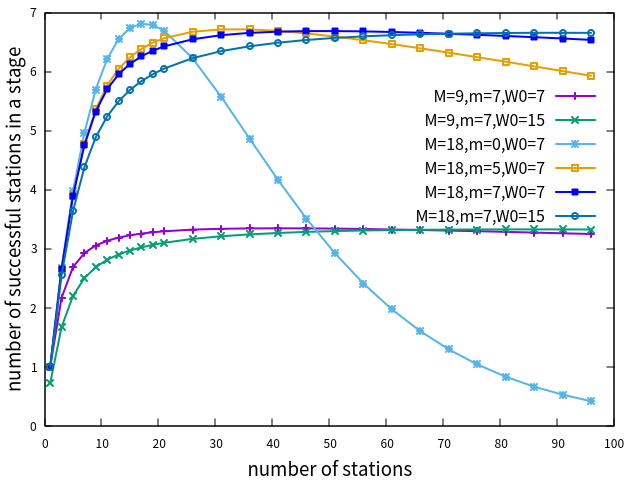
\includegraphics[scale=.54]{./figure/n_rule_ns_perf.png}
%\caption{$n_s$ versus number of stations}
%\label{fig_n_ns_val}
%\end{figure}
%
%\begin{figure}[!ht]
%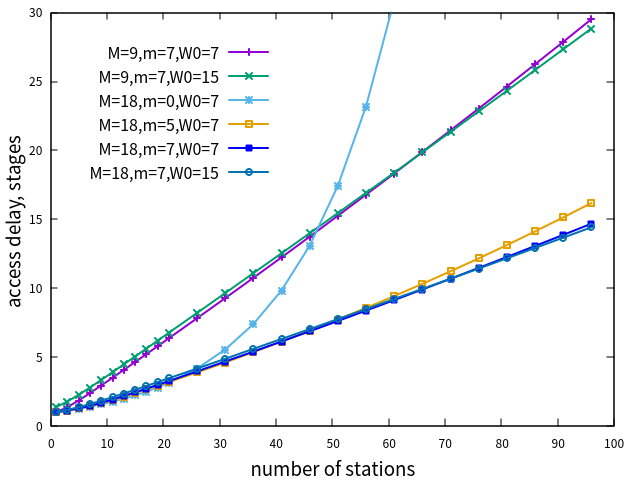
\includegraphics[scale=.54]{./figure/n_rule_delay_perf.png}
%\caption{Access Delay versus number of stations}
%\label{fig_n_delay_val}
%\end{figure}
